\documentclass[a4paper, 12pt]{article}
\usepackage[utf8]{inputenc}
\usepackage[english,russian]{babel}
\usepackage[warn]{mathtext}
\usepackage{graphicx}
\usepackage{float}
\usepackage{multirow}
\restylefloat{table}
\usepackage{amsmath}
\usepackage{floatflt}
\usepackage[T2A]{fontenc}
\usepackage[left=20mm, top=20mm, right=20mm, bottom=20mm, footskip=10mm]{geometry}

\tolerance 1414
\hbadness 1414
\emergencystretch 1.5em
\hfuzz 0.3pt        % размер максимального переполнения без warning'a
\widowpenalty=10000 % запрещает одиночную строку абзаца в начале страницы
\vfuzz \hfuzz
\raggedbottom       % если на странице мало содержимого, добавить пустое место в конце, а не в середине страницы



\begin{document}

\begin{titlepage}
	\centering
	\vspace{5cm}
	{\scshape\LARGE московский физико-технический институт (национальный исследовательский университет) \par}
	\vspace{6cm}
	{\scshape\Large Лабораторная работа 4.2.5 \par}
	{\huge\bfseries Когерентность света \par}
	\vspace{1cm}
	\vfill
\begin{flushright}
	{\large Б03-102}\par
	\vspace{0.3cm}
	{\LARGE Куланов Александр}
\end{flushright}
	

	\vfill


	Долгопрудный, 2023 г.
\end{titlepage}

\begin{itemize}
	\item \textbf{Цель работы:} измерить радиус когерентности и ширину спектра источника света
    \item \textbf{В работе используются:} лазер, галогенная лампа с блоком питания, объектив, оптические щели, микроскоп или видеокамера с PC
\end{itemize}

\section{Описание и теория}

Когерентность - характеристика в оптике, определяющая способность света к интерференции. Обычные тепловые источники света являются генераторами случайных полей, поэтому возникает проблема
согласованности световых колебаний в разных точках простанства в разное время. В работе ограничимся частным случаем: исследуем согласованность в точках с координатами $r_1$ и $r_2$ в
моменты времени $t_1$ и $t_2$. Колебания будем считать квазимонохроматическими с центральной частотой $\omega_0$. Поле считаем скалярным. Поле в точке $r$ в момент $t$ удобно записать 
в виде $A(r, t)e^{i\omega_0 t}$. Амплитуда $A$ мало меняется за период колебаний, равный порядка $10^{-15}$ с.

За меру когерентности светового поля в точках $r_1$ и $r_2$ в моменты $t_1$ и $t_2$ принимают нормированное среднее произведений амплитуд полей.

\begin{equation}
	\gamma=\frac{\overline{A\left(r_1, t_1\right) e^{i \omega_0 t_1} A^*\left(r_2, t_2\right) e^{-i \omega_0 t_2}}}{\sqrt{\overline{\left|A\left(r_1, t_1\right)\right|^2} \cdot \overline{\left|A\left(r_2, t_2\right)\right|^2}}}
\end{equation}

Черта означает усреднение по времени. Поле стационарно и время $T$ регистрации интенсивности полей много больше периода колебаний световых волн и длительности биений для любых
комбинаций частот в спектре:

\begin{equation}
	\overline{A\left(r_1, t_1\right) A^*\left(r_2, t_2\right)} \approx \frac{1}{T} \int_0^T A\left(r_1, t_1+t\right) A^*\left(r_2, t_2+t\right) d t
\end{equation}

Нас интересует частный случай, в котором исследуется согласованность колебаний в точках, лежащих в одной плоскости. Если световое поле является однородным в пространстве и его
статистические характеристики не зависят от времени, то функция когерентности $\gamma$ не зависит от $r_1, r_2$ и $t_1, t_2$, а зависит только от разности $\rho = |r_1 - r_2|$
и $\tau = t_2 - t_1$.

Входящая в (1) величина $\overline{|A(r,t)|^2}$ пропорциональная интенсивности света. Для выбранной пары точек интенсивность света будем считать постоянной и обозначим $\overline{|A|^2}$.
Тогда перепишем:

\begin{equation}
	\gamma(\rho, \tau)=e^{-i \omega_0 \tau} \frac{\overline{A(\boldsymbol{r}, t) A^*(\boldsymbol{r}+\rho, t+\tau)}}{\overline{|A|^2}}
\end{equation}

\section{Экспериментальная установка}

\begin{figure}[H]
    \centering
    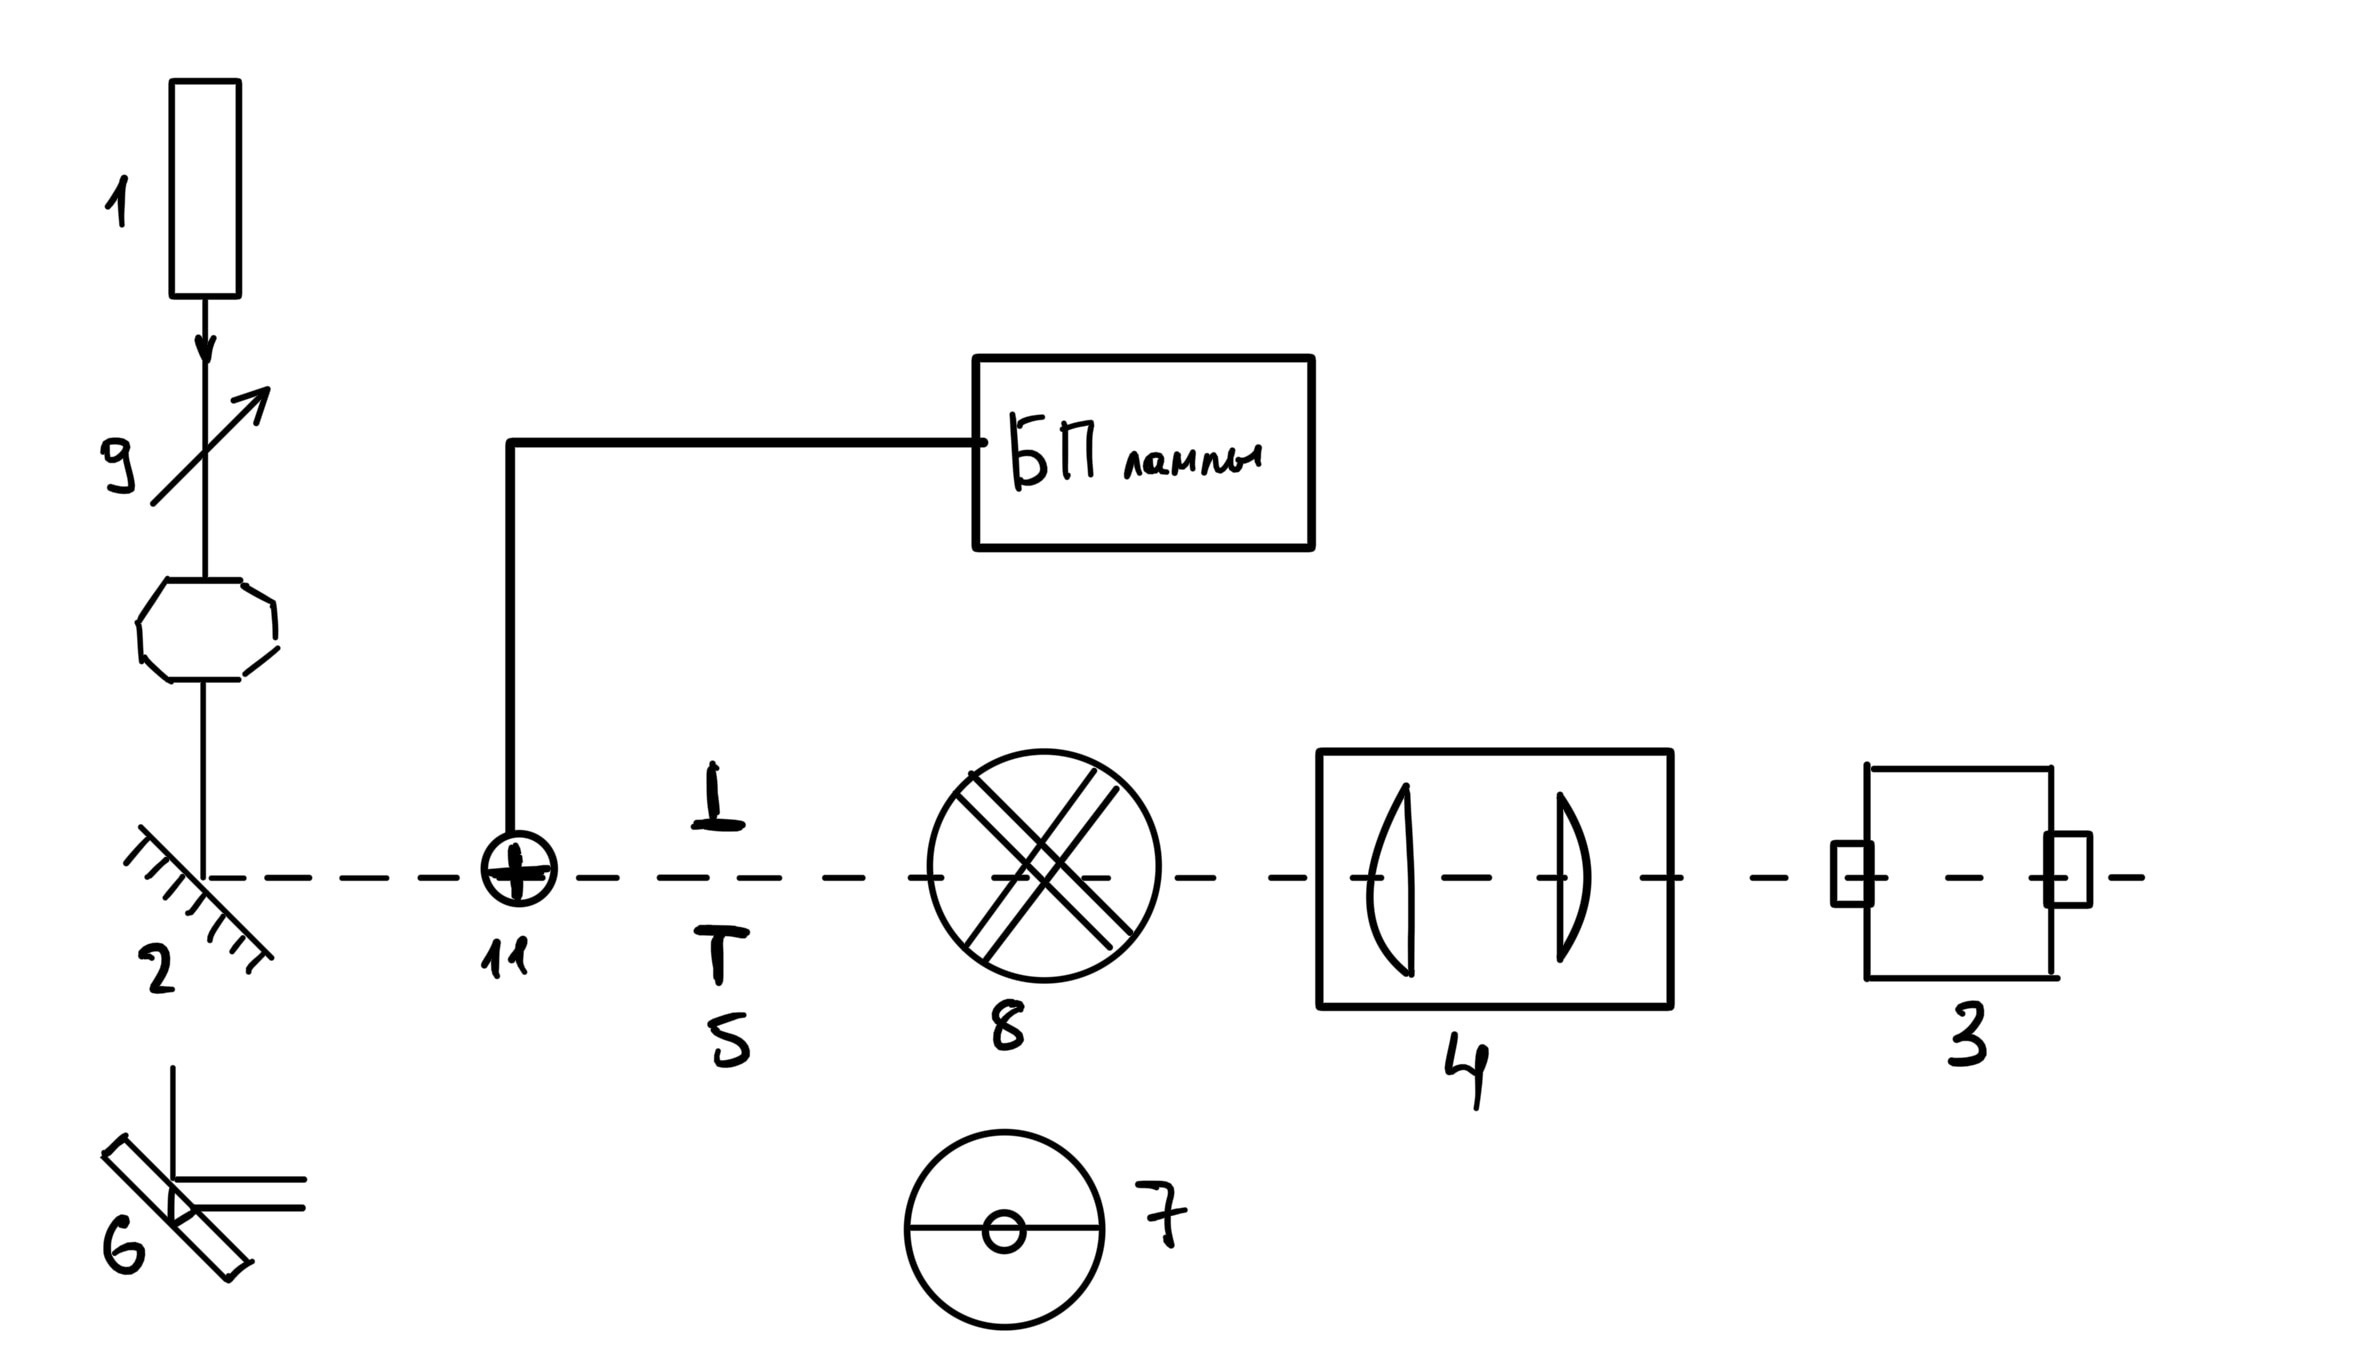
\includegraphics[width=1\textwidth]{set}
    \caption{Схема установки}
    \label{fig:set}
\end{figure}

 
\end{document}